\renewcommand{\theequation}{\theenumi}
\begin{enumerate}[label=\arabic*.,ref=\thesubsection.\theenumi]
\numberwithin{equation}{enumi}
%\chapter{The Optimum Receiver}

%\subsection{Problem}
\item


A right angled triangle looks like Fig. \ref{ch1_right}.
\begin{figure}[!ht]
\begin{center}
	
%\includegraphics[width=\columnwidth]{./figs/right_angle_tri.tex}
\resizebox{\columnwidth}{!}{
\begin{tikzpicture}[scale=2]%,cap=round,>=latex]

\coordinate [label=left:$B$] (A) at (-1.5cm,-1.0cm);
\coordinate [label=right:$C$] (C) at (1.5cm,-1.0cm);
\coordinate [label=above:$A$] (B) at (1.5cm,1.0cm);
\draw (A) -- node[sloped,above] {$\textrm{c}$} (B) -- node[above,xshift=2mm] {$\textrm{b}$} (C) -- node[below] {$\textrm{a}$} (A);

\draw (1.25cm,-1.0cm) rectangle (1.5cm,-0.75cm);
\tkzMarkAngle[size=0.5cm,color=black,mark=](C,A,B) 
\tkzLabelAngle[pos=0.65](C,A,B){$\theta$}
\end{tikzpicture}}
%\vspace*{-10cm}
\end{center}
\caption{Right Angled Triangle}
\label{ch1_right}	
\end{figure}
%\vspace*{-10cm}
with angles $\angle A,\angle B$ and $\angle C$ and sides $a, b$ and $c$.  The unique feature of this triangle is $\angle C$ which is defined to be $90^{\degree}$.
\item
	For simplicity, let the greek letter $\theta = \angle B$.  We have the following definitions.
\begin{equation}
\label{ch1_trig_defs}
\begin{matrix}
	\sin \theta = \frac{a}{c} & 	\cos \theta = \frac{b}{c} \\
	\tan \theta = \frac{b}{a} & \cot \theta = \frac{1}{\tan \theta} \\
	\csc \theta = \frac{1}{\sin \theta} & \sec \theta = \frac{1}{\cos \theta}
	\end{matrix}
\end{equation}
\end{enumerate}

\subsection{Sum of Angles}
\renewcommand{\theequation}{\theenumi}
\begin{enumerate}[label=\arabic*.,ref=\thesubsection.\theenumi]
\numberwithin{equation}{enumi}
\item 	In Fig. \ref{ch1_parallel_triangle}, the sum of all the angles on the top or bottom side of the straight line $XY$ is $180^{\degree}$.


\begin{figure}[!ht]
	\begin{center}
		\resizebox{\columnwidth}{!}{\begin{tikzpicture}
[scale=2,>=stealth,point/.style={draw,circle,fill = black,inner sep=0.5pt},]

\node (A) at (0, 0)[point,label=above right:$A$] {};
\node (Y) at (2, 0)[point,label=above right:$Y$] {};
\node (X) at (-2, 0)[point,label=above right:$X$] {};
\node (T) at (0, 1)[point,label=above right:$T$] {};
\node (V) at (-1.2, 1)[point,label=above right:$V$] {};
\node (C) at (0, -3)[point,label=below right:$C$] {};
\node (B) at (3.5, -3)[point,label=above right:$B$] {};
\draw (Y)--(A);
\draw (X)--(A);
\draw (T)--(A);
\draw (V)--(A);
\draw (C)--(A);
\draw (B)--(A);
\draw (B)--(C);

\tkzMarkAngle[size=.3](A,B,C)
\tkzMarkAngle[size=.3](V,A,X)
\tkzMarkAngle[size=.3](C,A,B)
\draw (-0.4,0.1) node{$\theta$};
\draw (3.1,-2.9)[label=below] node{$\theta$};
\tkzMarkRightAngle[size=.2](B,C,A)
\tkzMarkRightAngle[size=.2](C,A,X)

\node [below] at (1.7,-3.1) {$a$};
\node  at (-0.1,-1.5) {$b$};
\node at (2,-1.5) {$c$};

\end{tikzpicture}}
		%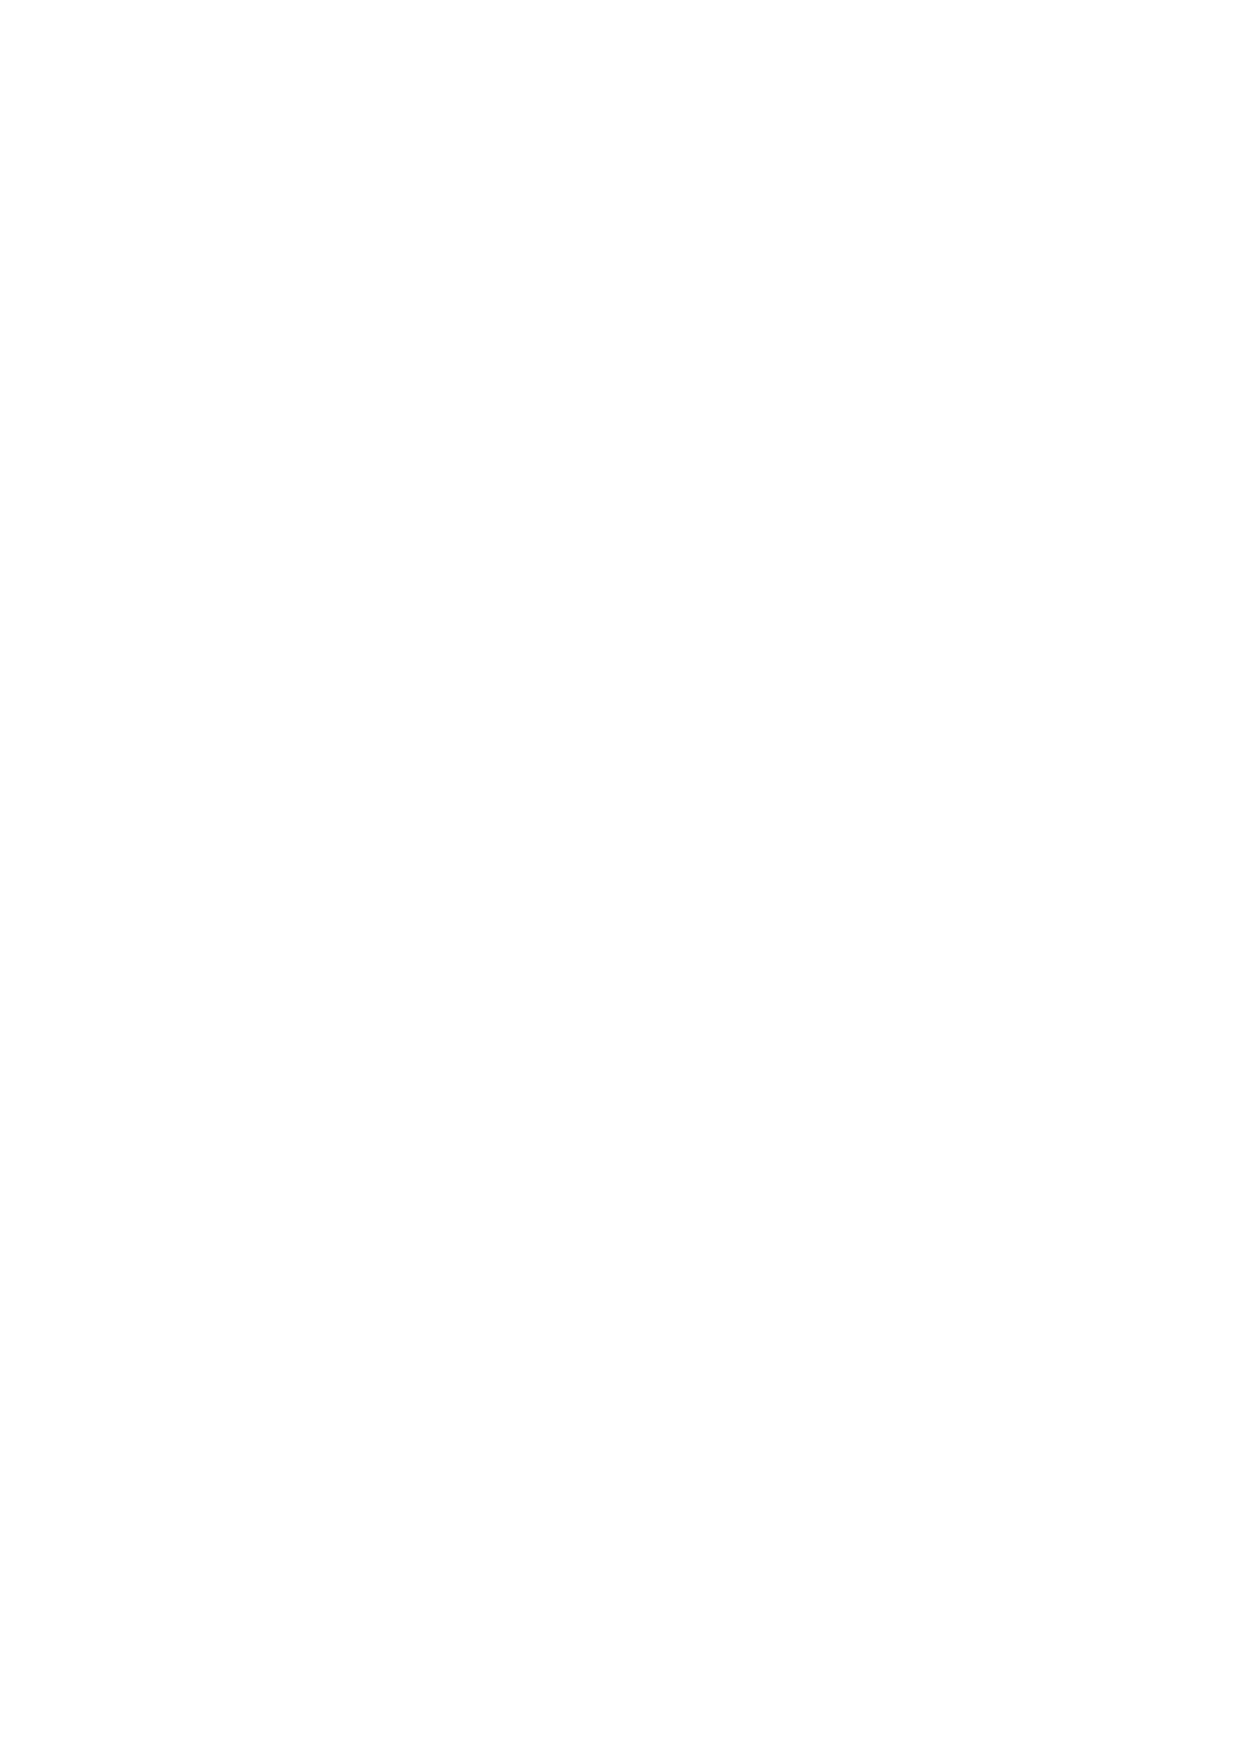
\includegraphics[width=\columnwidth]{./figs/ch1_parallel_triangle}
		%\vspace*{-10cm}
	\end{center}
	\caption{Sum of angles of a triangle}
	\label{ch1_parallel_triangle}	
\end{figure}



\item
In Fig. \ref{ch1_parallel_triangle}, the straight line making an angle of $90^{\degree}$ to the side $AC$ is said to be parallel to the side $BC$. Note there is an angle at $A$ that is equal to $\theta$.  This is one property of parallel lines.  Thus, $\angle YAZ = 90^{\degree}$.


\item
	Show that $\angle VAZ = 90^{\degree} - \theta$
		
	\solution Considering the line $XAZ$,
	\begin{align}
	\theta + 90^{\degree} + \angle VAZ &= 180^{\degree} \\
	\Rightarrow  \angle VAZ =  90^{\degree} - \theta
	\end{align}

\item
	\label{ch1_compl_angle}
	Show that $\angle BAC = 90^{\degree} - \theta$.
	
	\solution Consider the line $VAB$ and and use the approach in the previous problem.  Note that this implies that $\angle VAZ = \angle BAC$.  Such angles are known as vertically opposite angles. 
	 
\item
Sum of the angles of a triangle is equal to $180^{\degree}$
\end{enumerate}
\subsection{Baudhayana Theorem}
\renewcommand{\theequation}{\theenumi}
\begin{enumerate}[label=\arabic*.,ref=\thesubsection.\theenumi]
\numberwithin{equation}{enumi}



\item 	Using Fig. \ref{ch1_right}, show that
	\begin{equation}
	\cos \theta = \sin \brak{90^{\degree} - \theta}
	\end{equation}


\begin{figure}[!ht]
	\begin{center}
		
		%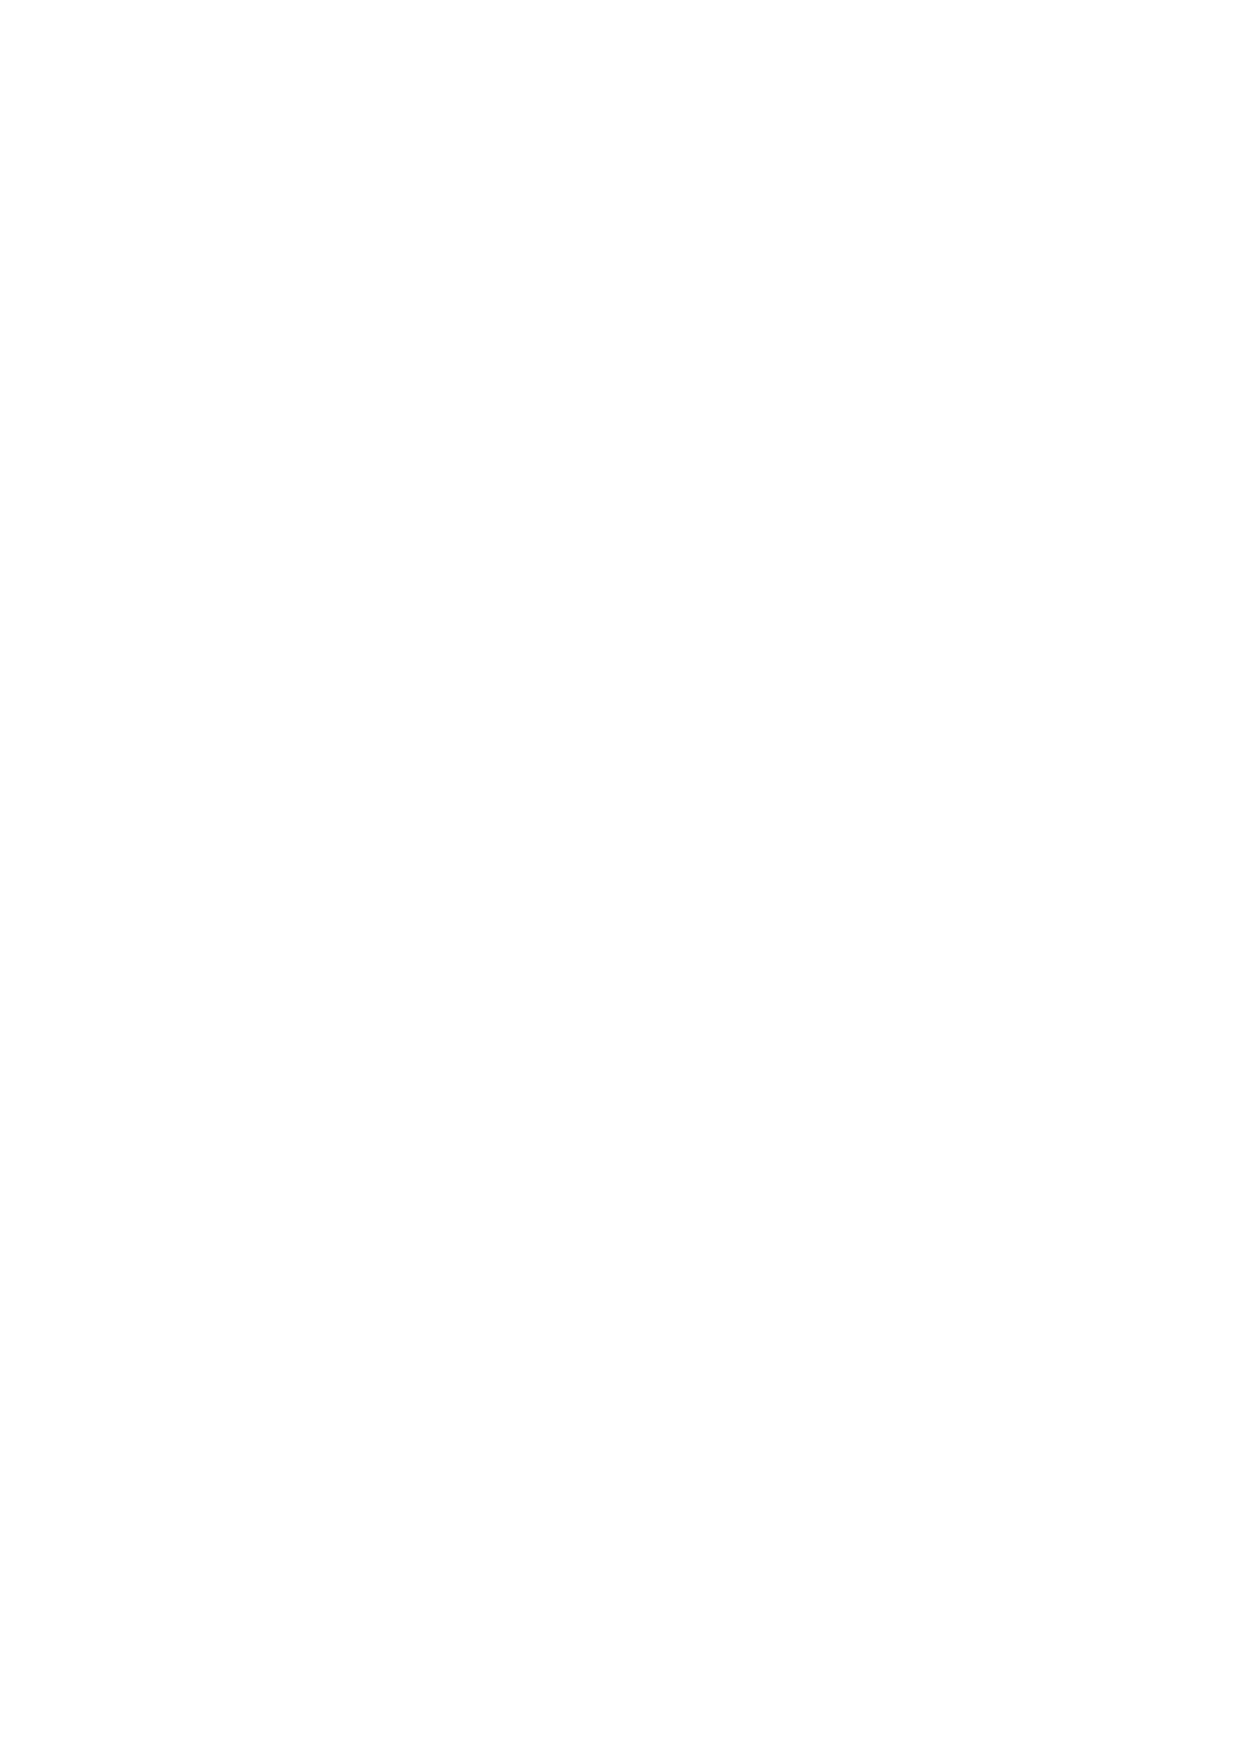
\includegraphics[width=\columnwidth]{./figs/ch1_budh_triangle}
		\resizebox{\columnwidth}{!}{
\begin{tikzpicture}
[scale=2,>=stealth,point/.style={draw,circle,fill = black,inner sep=0.5pt},]
\node (B) at (3, 0)[point,label=above right:$B$] {};
\node (A) at (-1, 3)[point,label=above right:$A$] {};
\node (C) at (-1, 0)[point,label=above left:$C$] {};

\draw (A)--(B);
\draw (B)--(C);
\draw (C)--(A);

\node (D) at (1, 1.5)[point,label= above right:$D$] {};
\draw (D)--(C);
\tkzMarkRightAngle[size=.2](B,C,A)
\tkzMarkRightAngle[size=.2](B,D,C)
\tkzMarkAngle[size=.3](A,B,C)
\tkzMarkAngle[size=.3](C,A,B)
\draw (2.6,0.12) node{$\theta$};
\draw (-.7,2.52) node{$90-\theta$};

\node [above] at (0.9,-0.2) {$a$};
\node [above] at (-1.1,1.2){$b$};
\node [below] at (0.9,1.9){$c$};
\end{tikzpicture}}
		%\vspace*{-10cm}
	\end{center}
	\caption{Baudhayana Theorem}
	\label{ch1_budh_triangle}	
\end{figure}


\solution From Problem \ref{ch1_compl_angle} and  \eqref{ch1_trig_defs}
%
\begin{equation}
\label{eq:tri_90-ang}
	\cos \brak{90^{\degree}-\theta} = \frac{b}{c} = \sin \theta
\end{equation}
%
\item
Using Fig. \ref{ch1_budh_triangle}, show that 
%
\begin{equation}
\label{ch1_budh_basic}
c = a \cos \theta + b \sin \theta
\end{equation}
%

\solution We observe that
%
\begin{align}
BD &= a \cos \theta \\
AD &= b \cos\brak{90-\theta} = b \sin \theta \quad \brak{\text{From} \quad \eqref{ch1_compl_angle}}
\end{align}
%
Thus,
\begin{equation}
BD + AD = c = a \cos \theta + b \sin \theta
\end{equation}
\item
From \eqref{ch1_budh_basic}, show that
%
\begin{equation}
%
\label{eq:tri_sin_cos_id}
\sin ^2 \theta + \cos ^2 \theta = 1
\end{equation}


%
\solution Dividing both sides of \eqref{ch1_budh_basic} by $c$, 
\begin{align}
1 &= \frac{a}{c}\cos\theta + \frac{b}{c}\sin\theta\\
\Rightarrow &\sin ^2 \theta + \cos ^2 \theta = 1 \quad \brak{\text{from} \quad \eqref{ch1_trig_defs}}
\end{align}

\item
	Using \eqref{ch1_budh_basic}, show that
	\begin{equation}
	\label{ch1_Baudhayana_them}
	c^2 = a^2 + b^2
	\end{equation}
	\eqref{ch1_Baudhayana_them} is known as the Baudhayana theorem.  It is also known as the Pythagoras theorem.

\solution From \eqref{ch1_budh_basic},
\begin{align}
c &= a\frac{a}{c} + b \frac{b}{c} \quad \brak{\text{from} \quad \eqref{ch1_trig_defs}}\\
\Rightarrow c^2 &= a^2 + b^2
\end{align}
\end{enumerate}
\subsection{Area of a Triangle}
\renewcommand{\theequation}{\theenumi}
\begin{enumerate}[label=\arabic*.,ref=\thesubsection.\theenumi]
\numberwithin{equation}{enumi}
%



\item
	The area of the rectangle $ACBD$ shown in Fig. \ref{ch2_sq_ar} is defined as $ab$. Note that all the angles in the rectangles are $90^{\degree}$
%	\label{ch2_sq_ar}

\begin{figure}[!ht]
	\begin{center}
		
		%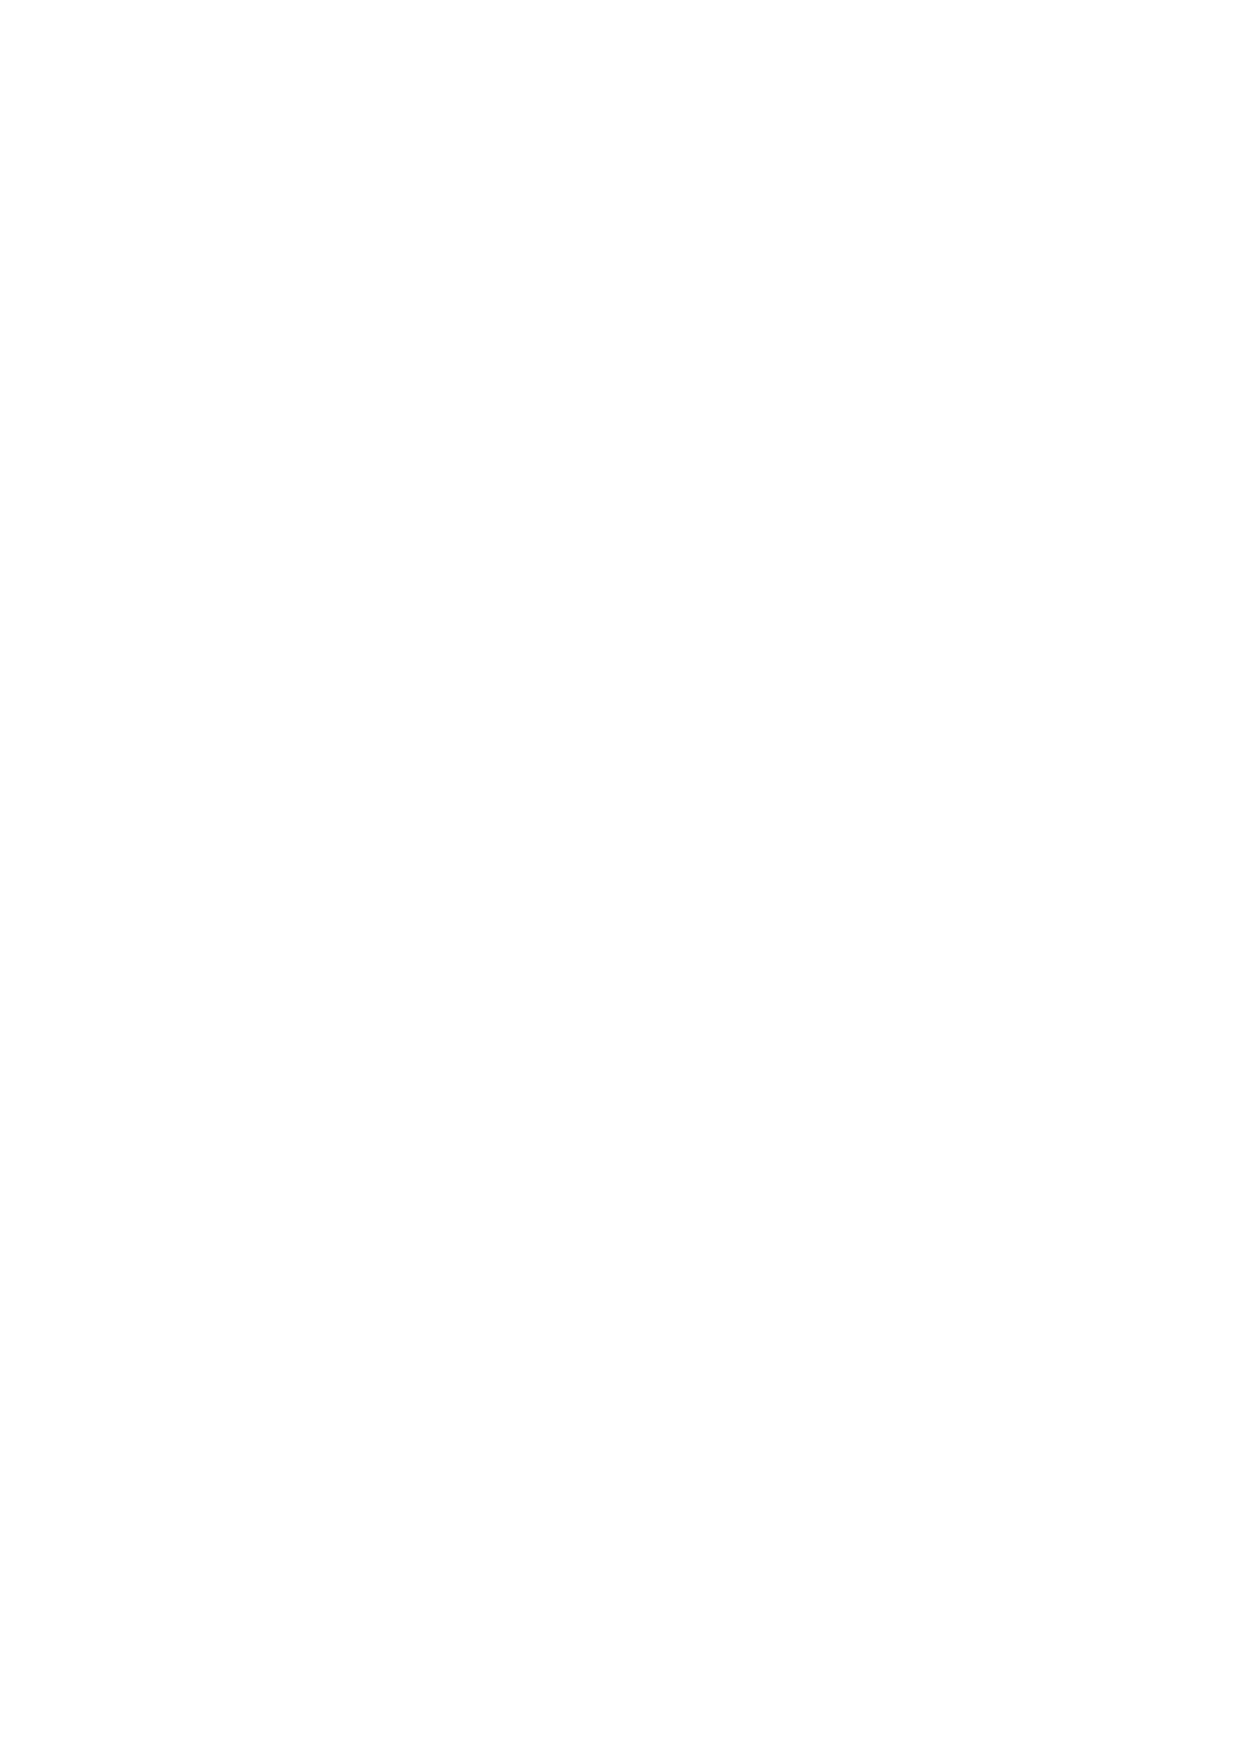
\includegraphics[width=\columnwidth]{./figs/ch2_sq_ar}
		%\vspace*{-10cm}
		\resizebox{\columnwidth}{!}{\begin{tikzpicture}
[scale=2,>=stealth,point/.style={draw,circle,fill = black,inner sep=0.5pt},]

\node (C) at (0, 0)[point,label=below left:$C$] {};
\node (A) at (0, 3)[point,label=above left:$A$]{};
\node (D) at (3, 3)[point,label=above right:$D$]{};
\node (B) at (3, 0)[point,label=below right:$B$]{};

\draw (C)--(A);
\draw (A)--(D);
\draw (D)--(B);
\draw (B)--(C);
\draw (B)--(A);
\tkzMarkRightAngle[size=.2](B,C,A)
\tkzMarkRightAngle[size=.2](A,D,B)

\node [below] at (1.5,0) {$a$};
\node [above] at (1.5,3) {$a$};
\node [left] at (0,1.5) {$b$};
\node [right] at (3,1.5) {$b$};

\end{tikzpicture}}
	\end{center}
	\caption{Area of a Right Triangle}
	\label{ch2_sq_ar}	
\end{figure}

\item
	The area of the two triangles constituting the rectangle is the same.
	\label{ch2_triang_eq}

\item
	The area of the rectangle is the sum of the areas of the two triangles inside.
	\label{ch2_triang_sum}


\item
\label{prob:ch2_triang_area}
	Show that the area of $\Delta ABC$ is $\frac{ab}{2}$

\begin{figure}[!ht]
	\begin{center}
		
		%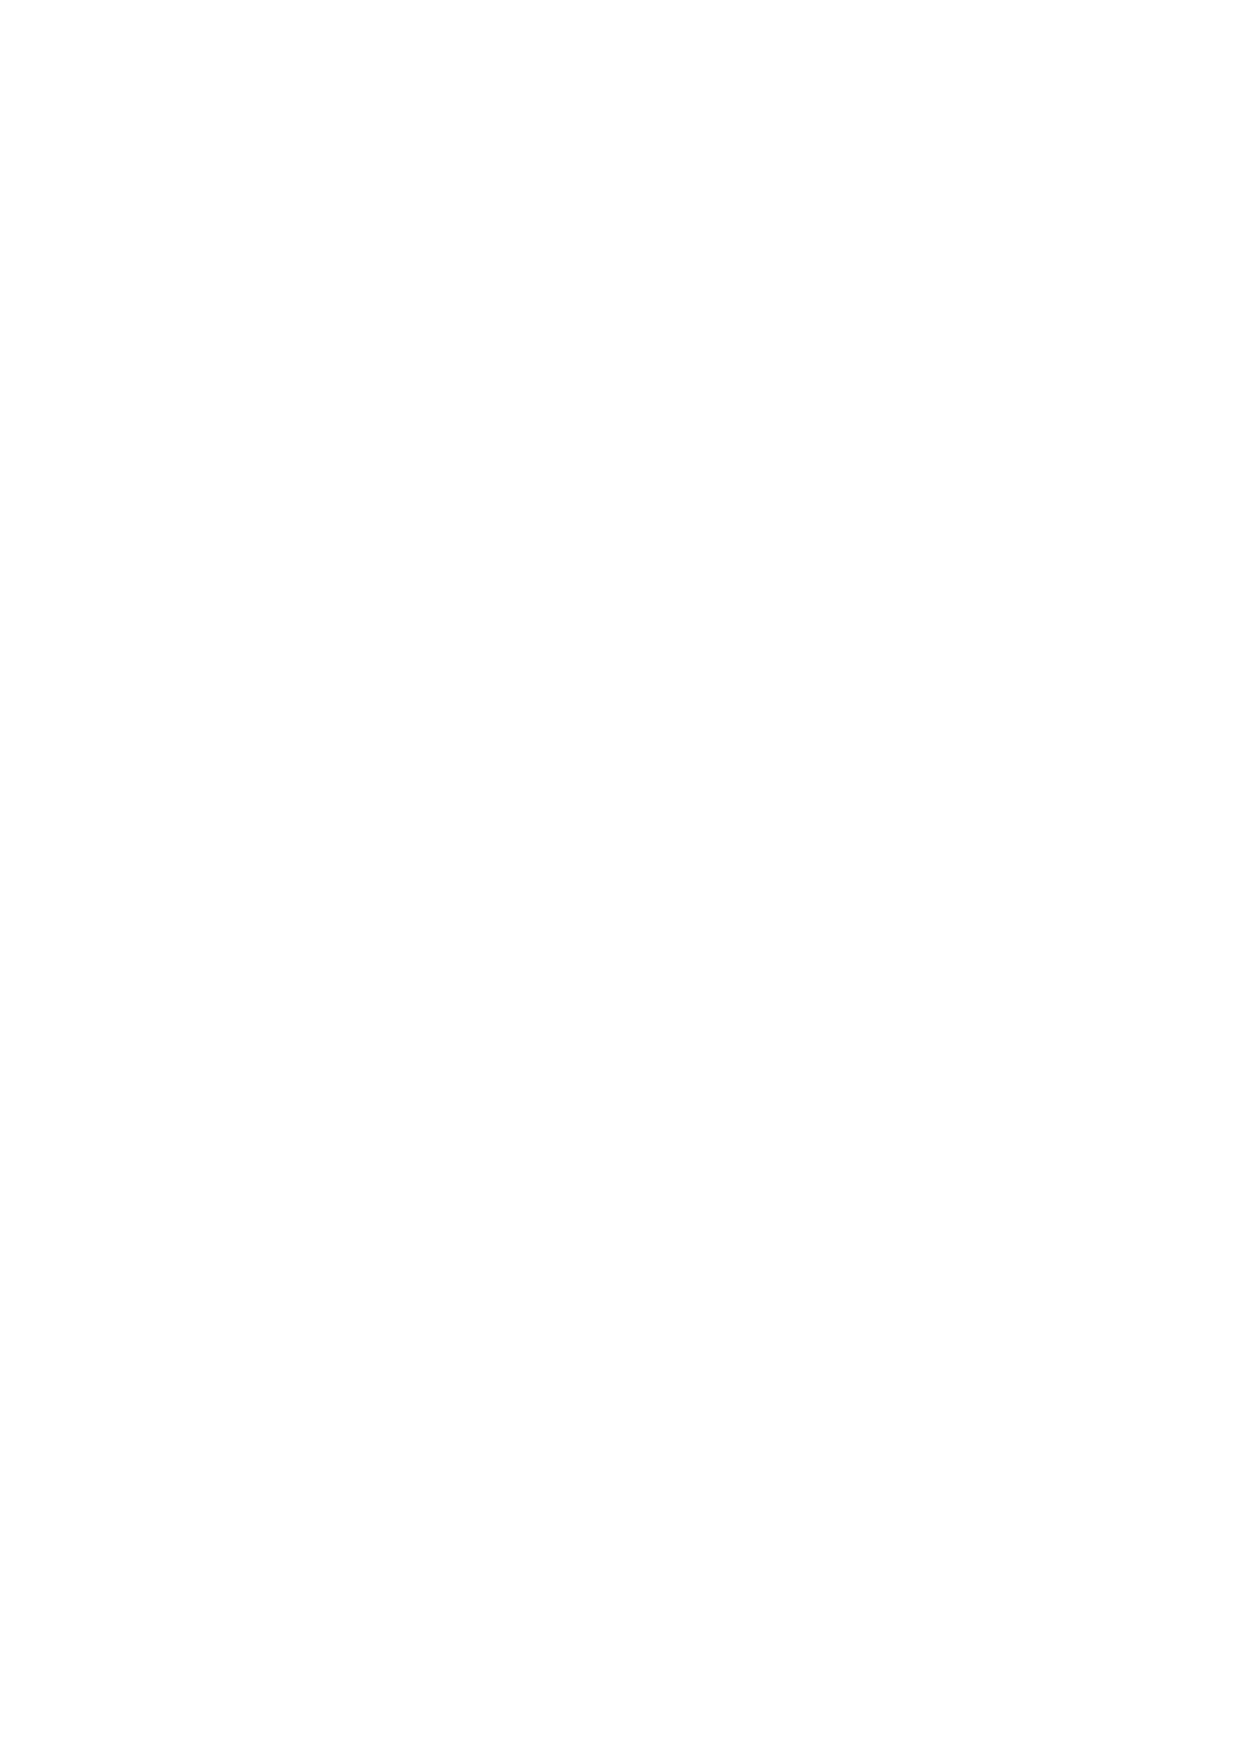
\includegraphics[width=\columnwidth]{./figs/ch2_triang_ar}
		%\vspace*{-10cm}
		\resizebox{\columnwidth}{!}{\begin{tikzpicture}
[scale=2,>=stealth,point/.style={draw,circle,fill = black,inner sep=0.5pt},]

\node (D) at (0, 0)[point,label=below :$D$] {};
\node (A) at (0, 3)[point,label=above :$A$]{};
\node (B) at (-3, 0)[point,label=below left:$B$]{};
\node (C) at (3, 0)[point,label=below right:$C$]{};

\draw (D)--(B);
\draw (B)--(A);
\draw (A)--(C);
\draw (C)--(D);
\draw (D)--(A);

\tkzMarkRightAngle[size=.2](A,D,C)

\node [below] at (0,-0.3) {$a$};
\node [below] at (-1.5,0) {$x$};
\node [below] at (1.5, 0) {$y$};
\node [below] at (0.1,1.5) {$h$};
\node [above] at (-1.5,1.5){$c$};
\node [above] at (1.5,1.5){$b$};

\end{tikzpicture}}
	\end{center}
	\caption{Area of a Triangle}
	\label{ch2_triang_ar}	
\end{figure}

\solution From\eqref{ch2_triang_sum},
\begin{equation}
\label{ch2_triang_ar_1}
ar\brak{ABCD} = ar\brak{ACB} + ar\brak{ADB}
\end{equation}
Also from \eqref{ch2_triang_eq},
\begin{equation}
\label{ch2_triang_ar_2}
ar\brak{ACB} = ar\brak{ADB}
\end{equation}
From \eqref{ch2_triang_ar_1} and \eqref{ch2_triang_ar_2},
\begin{align}
2ar\brak{ACB} &= ar\brak{ABCD} = ab \brak{\text{from} \quad \eqref{ch2_sq_ar}}
\\
\Rightarrow ar\brak{ACB} &= \frac{ab}{2}
\end{align}

\item
	Show that the area of $\Delta ABC$ in Fig. 	\ref{ch2_triang_ar}	is $\frac{1}{2}ah$.


\solution In Fig. \ref{ch2_triang_ar},
\begin{align}
ar\brak{\Delta ADC} &= \frac{1}{2}hy \\
ar\brak{\Delta ADB} &= \frac{1}{2}hx 
\end{align}
Thus,
\begin{align}
ar\brak{\Delta ABC} &= ar\brak{\Delta ADC} + ar\brak{\Delta ADB} \\
&= \frac{1}{2}hy + \frac{1}{2}hx = \frac{1}{2}h\brak{x+y} \\
&= \frac{1}{2}ah
\end{align}
\item
\label{prob:tri_area_sin}
	Show that the area of $\Delta ABC$ in Fig. 	\ref{ch2_triang_ar}	is $\frac{1}{2}ab \sin C$.

\solution We have
%
\begin{equation}
ar\brak{\Delta ABC} = \frac{1}{2}ah = \frac{1}{2}ab\sin C \quad \brak{\because \quad h = b \sin C}.
\end{equation}
%
\item
	Show that 
	\begin{equation}
	\frac{\sin A}{a} = \frac{\sin B}{b} = \frac{\sin C}{c}
	\end{equation}

\solution Fig. \ref{ch2_triang_ar} can be suitably modified to obtain 
\begin{equation}
ar\brak{\Delta ABC} = \frac{1}{2}ab\sin C = \frac{1}{s}bc\sin A = \frac{1}{2}ca\sin B
\end{equation}
Dividing the above by $abc$, we obtain
	\begin{equation}
\label{eq:tri_sin_form}
	\frac{\sin A}{a} = \frac{\sin B}{b} = \frac{\sin C}{c}
	\end{equation}
This is known as the sine formula.	
%
\item
In Fig. \ref{ch2_cosine_formula}, show that
%
\begin{equation}
\label{eq:tri_cos_form}
\cos A = \frac{b^2+c^2-a^2}{2bc}
\end{equation}
%
\

\begin{figure}[!ht]
	\begin{center}
		
		%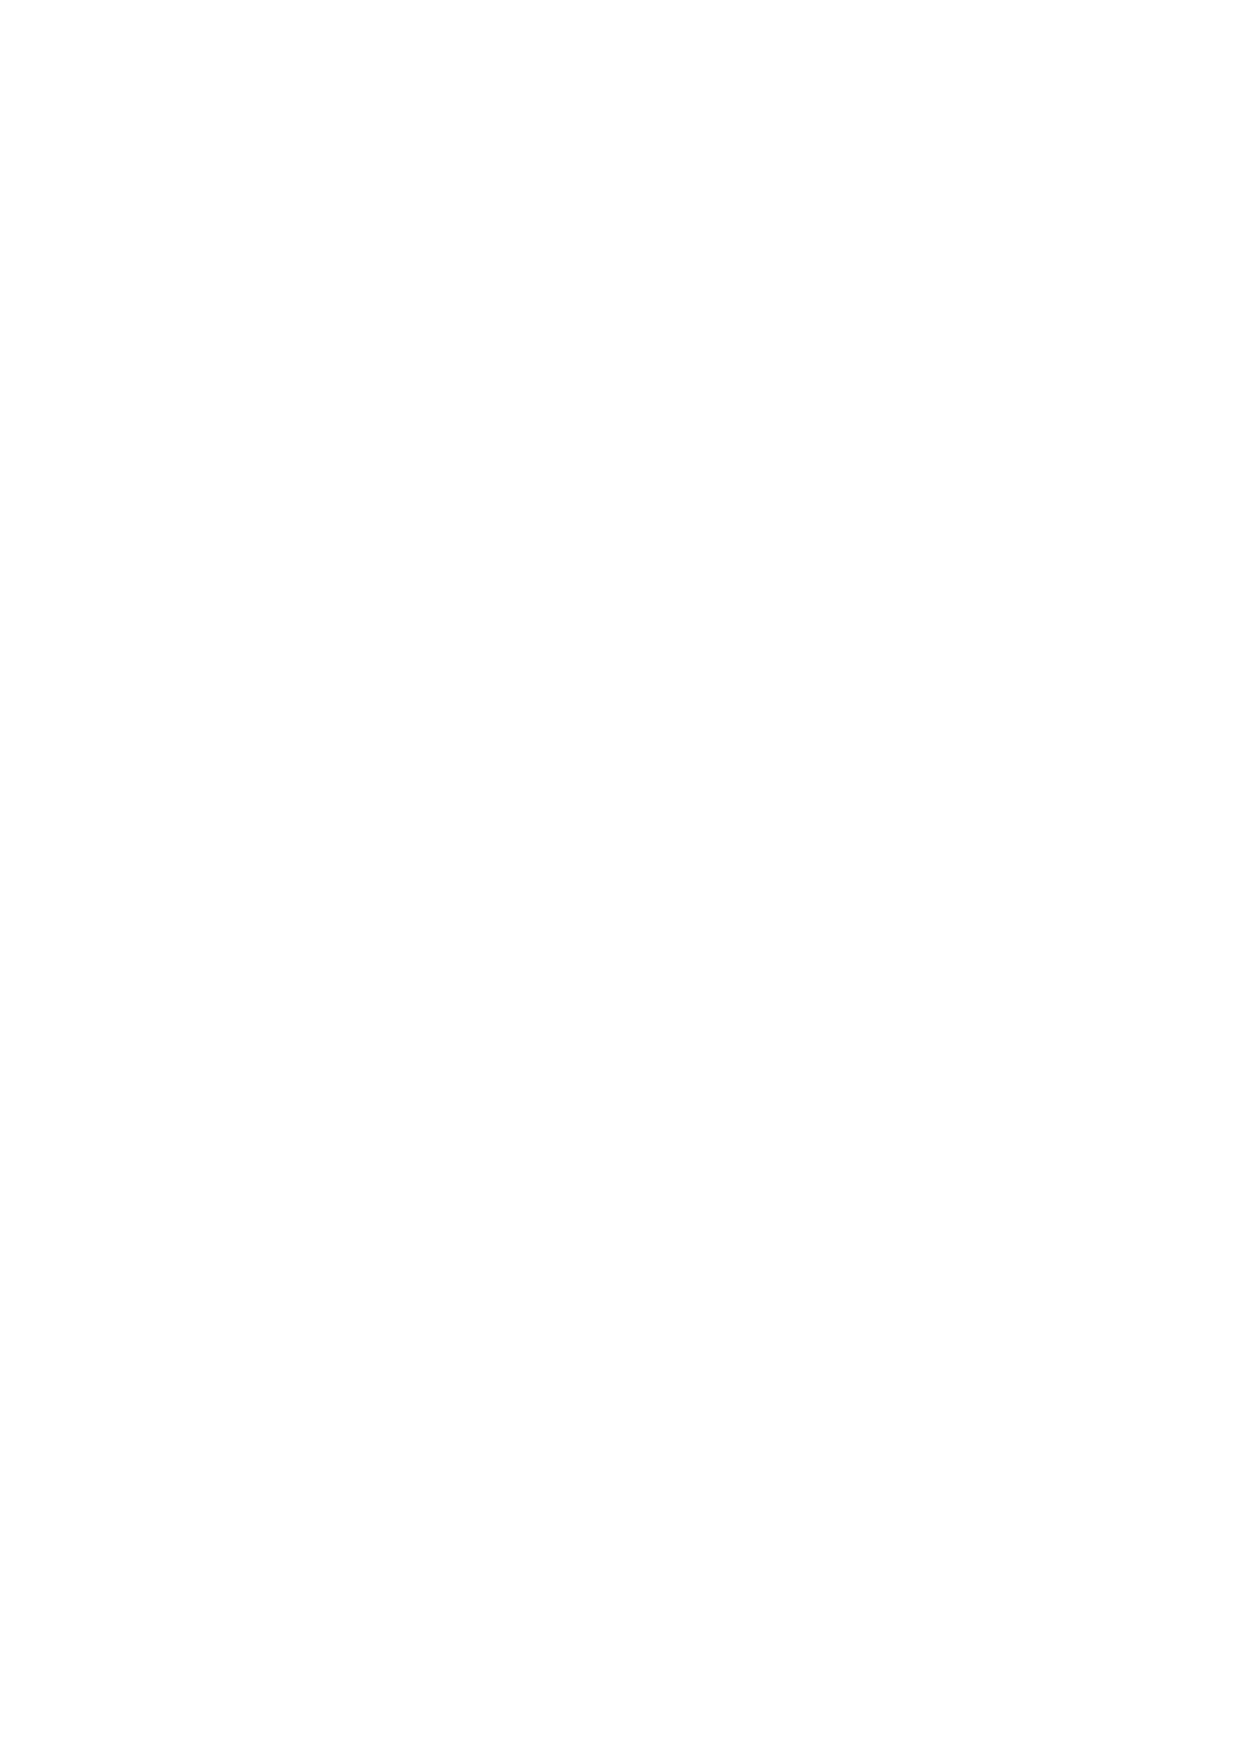
\includegraphics[width=\columnwidth]{./figs/ch2_triang_ar}
		%\vspace*{-10cm}
		\resizebox{\columnwidth}{!}{\begin{tikzpicture}
[scale=2,>=stealth,point/.style={draw,circle,fill = black,inner sep=0.5pt},]

\node (D) at (0, 0)[point,label=below :$D$] {};
\node (A) at (0, 3)[point,label=above :$A$]{};
\node (B) at (-3, 0)[point,label=below left:$B$]{};
\node (C) at (3, 0)[point,label=below right:$C$]{};

\draw (D)--(B);
\draw (B)--(A);
\draw (A)--(C);
\draw (C)--(D);
\draw (D)--(A);

\tkzMarkRightAngle[size=.2](A,D,C)

\node [below] at (0,-0.3) {$a$};
\node [below] at (-1.5,0) {$x$};
\node [below] at (1.5, 0) {$y$};
\node [below] at (0.1,1.5) {$h$};
\node [above] at (-1.5,1.5){$c$};
\node [above] at (1.5,1.5){$b$};

\end{tikzpicture}}
	\end{center}
	\caption{The cosine formula}
	\label{ch2_cosine_formula}	
\end{figure}

\solution From the figure, the first of the following equations
%
\begin{align}
a &= b \cos C + c \cos B \\
b &= c \cos A + a \cos C \\
c &= b \cos A + a \cos B
\end{align}
%
is obvious and the other two can be similarly obtained.  The above equations can be expressed in matrix form as
%
\begin{equation}
\begin{pmatrix}
0 & c & b \\
c & 0 & a \\
b & a & 0
\end{pmatrix}
\begin{pmatrix}
\cos A \\
\cos B \\
\cos C
\end{pmatrix}
= 
\begin{pmatrix}
a\\
b\\
c
\end{pmatrix}
\end{equation}
%
Using the properties of determinants,
%
\begin{align}
\cos A &= \frac{
\begin{vmatrix}
a & c & b \\
b & 0 & a \\
c & a & 0
\end{vmatrix}
	}
	{
\begin{vmatrix}
0 & c & b \\
c & 0 & a \\
b & a & 0
\end{vmatrix}
	}
	=\frac{ab^2 + ac^2 - a^3}{abc + abc} 
\\
&= \frac{b^2 + c^2 - a^2}{2abc}
\end{align}
%
\item Find Hero's formula for the area of a triangle.
\\
\solution 
%In Fig. \ref{fig:rt_triangle}, from Baudhayana's theorem, 
%\begin{align}
%\label{eq:tri_geo_baudh}
%b^2 = a^2+c^2 &
%\\
%=b^2\cos^2C+b^2\sin^2C &
%\\
%\implies \cos^2C+\sin^2C &= 1
%\end{align}
%
%In Fig. \ref{fig:tri_const_ex_cos_form}, 
From \eqref{prob:tri_area_sin}, the area of $\triangle ABC$ is 
{\footnotesize
\begin{align}
\label{eq:tri_geo_area_sin_form}
 \frac{1}{2}ab\sin C
%\\
&=\frac{1}{2}ab\sqrt{1-\cos^2C} 
\quad \brak{\text{from } \eqref{eq:tri_sin_cos_id}
%\eqref{eq:tri_geo_baudh}
}
\\
&=\frac{1}{2}ab\sqrt{1-\brak{\frac{a^2+b^2-c^2}{2ab}}^2} \brak{\text{from } \eqref{eq:tri_cos_form}
}
\\
&=\frac{1}{4}\sqrt{\brak{2ab}^2-\brak{a^2+b^2-c^2}}
\\
&=\frac{1}{4}\sqrt{\brak{2ab+a^2+b^2-c^2}\brak{2ab-a^2-b^2+c^2}}
\\
&= \frac{1}{4}\sqrt{\cbrak{\brak{a+b}^2-c^2}\cbrak{c^2-\brak{a-b}^2}}
\\
&= \frac{1}{4}\sqrt{\brak{a+b+c}\brak{a+b-c}\brak{a+c-b}\brak{b+c-a}}
\label{eq:tri_ex_hero_temp}
\end{align}
}
Substituting 
%
\begin{align}
s=\frac{a+b+c}{2}
\end{align}
%
in \eqref{eq:tri_ex_hero_temp}, the area of $\triangle ABC$ is 
%
\begin{align}
\label{eq:tri_hero}
\sqrt{s\brak{s-a}\brak{s-b}\brak{s-c}}
\end{align}
%
This is known as Hero's formula.
\end{enumerate}


